\chapter{Introduction}

Deforestation has long been a concern throughout tropical South America. However, this process of land use/land cover (LULC) change from forest to other uses has been increasingly recognized in subtropical South America as a significant source of environmental degradation. Understanding the complex dynamics of subtropical deforestation is crucial given the prominent role of forests in debates about climate change, conservation, and the protection of endangered species \autocites{geist2002proximate}{zak2004do-subtropical}{bonnie2000counting}{houghton1994the-worldwide}{sala2000global}.

Currently, many perceive growing demand for agricultural land---particularly land for soybeans---to be one of the greatest pressures on South American subtropical forests \autocites{pengue2005transgenic}{grau2005agriculture}{altieri2006gm-soybean:}. Remote sensing has given researchers a tool to classify land cover and measure deforestation, but the often used multi-spectral or multi-temporal image classification techniques require extensive ground truth information for the accurate classification of common crop types using widely-available data. Therefore, getting a complete picture of the dynamics of deforestation, including an understanding of agricultural pressures on forests, requires a significant expense for high spatial or high spectral resolution data, or for field time gathering training site data. The development of a tool that can efficiently and effectively extract crop types using widely-available imagery would be of value to the field.

The primary goal of my thesis is to develop and test a a phenological classification algorithm that can identify and extract crop types from a multi-date vegetation index sequence assembled using free and accessible data from the National Aeronautics and Space Administration’s (NASA) Moderate Resolution Imaging Spectroradiometer (MODIS) platform. I will first test the algorithm using five small test areas from across the state of Kansas using the U.S. Department of Agriculture's (USDA) crop data layer (CDL) as ground truth to derive reference crop phenologies and to test the accuracy of the classification. Then, once I have determined the best parameters for use, I will apply the method to the Department of Pellegrini in Santiago del Estero, Argentina (Fig. \ref{fig:pellegrini}) during the 2013-2014 growing season to examine the method's applicability in subtropical South America.

\begin{figure}[H]
  \centering
  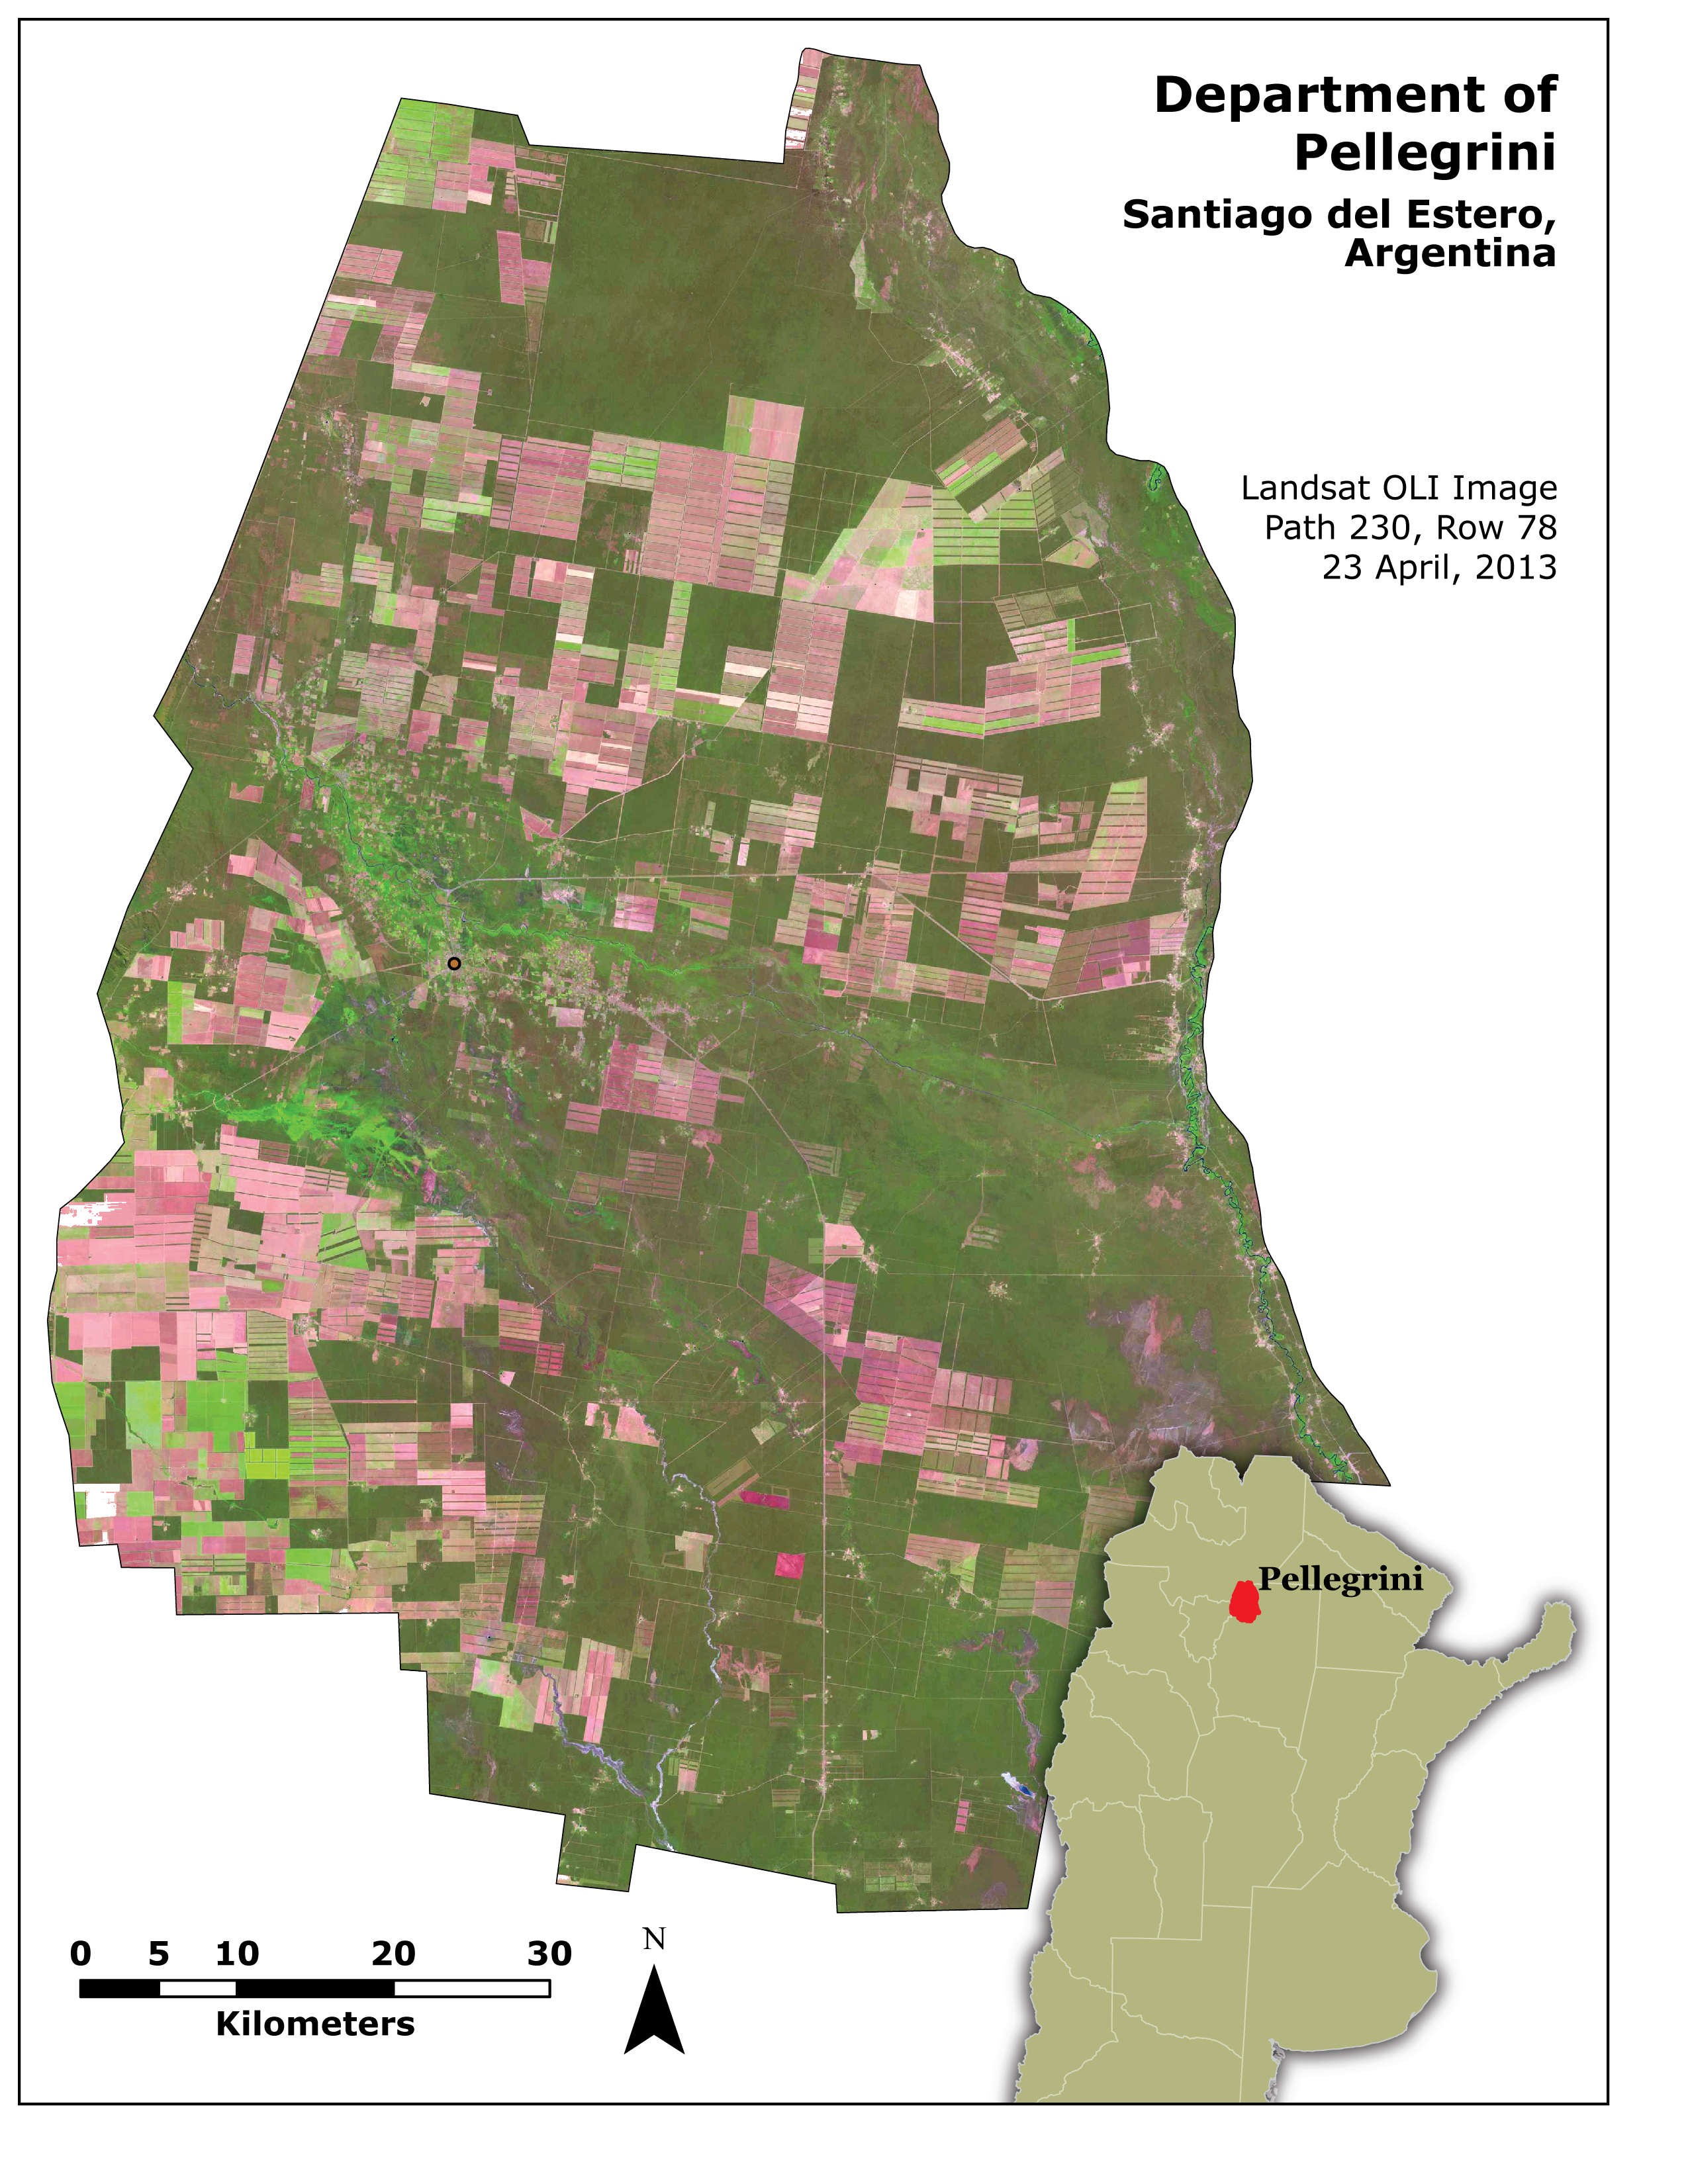
\includegraphics[width=.7\textwidth]{Graphics/pellegrini2.png}
  \caption{The department of Pellegrini, Santiago Del Estero, Argentina.}
  \label{fig:pellegrini}
\end{figure}
